\chapter{\texorpdfstring{\textbf{Introduzione}}{Capitolo 1 - Introduzione}}\label{capitolo-1-introduzione}

\section{\texorpdfstring{\textbf{Contesto e Motivazione della
Ricerca}}{Contesto e Motivazione della Ricerca}}\label{contesto-e-motivazione-della-ricerca}
\textit{Nota di trasparenza metodologica: Questa ricerca presenta un framework 
teorico sviluppato attraverso analisi della letteratura e validazione 
simulativa. Non sono stati raccolti dati diretti da organizzazioni reali 
per ragioni di confidenzialità e sicurezza. Tutti i risultati presentati 
derivano da modelli e simulazioni basati su parametri pubblicamente disponibili.}
\subsection{\texorpdfstring{\textbf{La Complessità Sistemica
della GDO
Moderna}}{La Complessità Sistemica della GDO Moderna}}\label{la-complessituxe0-sistemica-della-gdo-moderna}

Il settore della Grande Distribuzione Organizzata in Italia gestisce
un'infrastruttura tecnologica di complessità paragonabile a quella di
operatori di telecomunicazioni o servizi finanziari; con 27.432 nodi computazionali distribuiti\supercite{istat2024struttura} che processano 521 transazioni al secondo (TPS)\supercite{federdistribuzione2024mappa} con vincoli di latenza P99 < 50 ms (ovvero il 99\% delle transazioni risponde entro 50 ms) e requisiti di disponibilità definiti da \textbf{SLA (Service Level Agreement)} multi-livello (Tier 1: 99.99\%, Tier 2: 99.95\%, Tier 3: 99.9\%), la GDO rappresenta un caso di studio unico per l'ingegneria dei sistemi distribuiti mission-critical,dove l'infrastruttura deve garantire livelli di disponibilità differenziati secondo 
standard industriali consolidati:
\begin{itemize}
    \item Tier 1: disponibilità 99.99\% (52.56 minuti di downtime annuo massimo)
    \item Tier 2: disponibilità 99.95\% (262.8 minuti di downtime annuo massimo)  
    \item Tier 3: disponibilità 99.9\% (525.6 minuti di downtime annuo massimo)
\end{itemize}

La formula per calcolare il down-time massimo ammissibile è:\\
Downtime\_annuo = (1 - SLA) × 365 × 24 × 60 minuti

Inoltre l'infrastruttura IT della GDO moderna deve garantire simultaneamente
continuità operativa H24 in ambienti fisicamente distribuiti, processare
volumi transazionali con picchi del 300-500\% durante eventi
promozionali (come il Natale, Black Friday, etc.) \supercite{verizon2024dbir}, proteggere dati sensibili di pagamento e personali sotto multiple normative, integrare sistemi legacy con tecnologie
cloud-native, e gestire la convergenza tra \textbf{Information Technology (IT)} e
\textbf{Operational Technology (OT)}.

La complessità di questi requisiti è amplificata dalla natura
distribuita delle operazioni; ogni punto vendita rappresenta
essenzialmente un nodo computazionale autonomo che deve mantenere
sincronizzazione con i sistemi centrali, garantire operatività anche in
caso di disconnessione temporanea, e rispettare stringenti requisiti di
sicurezza e compliance.

Questa architettura distribuita crea sfide uniche in termini di gestione
della consistenza dei dati, propagazione degli aggiornamenti, e
contenimento delle minacce informatiche.

\subsection{\texorpdfstring{\textbf{L'Evoluzione del Panorama
Tecnologico e
Normativo}}{L'Evoluzione del Panorama Tecnologico e Normativo}}\label{levoluzione-del-panorama-tecnologico-e-normativo}

Il settore della GDO sta attraversando una trasformazione profonda
guidata da tre trend convergenti che ridefiniscono i paradigmi
architetturali tradizionali.

- Il primo trend riguarda \textbf{la trasformazione infrastrutturale}:
il passaggio da data center tradizionali ad architetture cloud-ibride,
documentato nel report di settore del 2024\supercite{gartner2024marketguide}, indica che il 67\% delle
organizzazioni GDO europee ha iniziato processi di migrazione verso
modelli cloud-first\supercite{eurostat2024digital}.

Questa transizione non rappresenta semplicemente uno spostamento di
carico di lavoro, ma richiede un ripensamento fondamentale dei modelli
operativi, delle strategie di sicurezza e dei processi di governance.

- Il secondo trend concerne \textbf{l'evoluzione delle minacce
informatiche}: l'incremento del 312\% negli attacchi ai sistemi retail
tra il 2021 e il 2023\supercite{mandiant2025mtrends} e l'emergere di attacchi cyber-fisici che possono
compromettere sistemi OT come refrigerazione e \textbf{HVAC (Heating,
Ventilation, and Air Conditioning)} richiedono un ripensamento radicale
delle strategie di sicurezza.

Non è più sufficiente proteggere i dati; è necessario garantire la
sicurezza dell'intera catena operativa, dal data center al punto
vendita, dal sistema informativo all'infrastruttura fisica.

- Il terzo trend riguarda \textbf{la crescente complessità normativa}:
l'entrata in vigore simultanea del \textbf{Payment Card Industry Data
Security Standard (PCI-DSS)} versione 4.0 nel marzo 2024, gli
aggiornamenti continui del \textbf{General Data Protection Regulation
(GDPR)} e l'implementazione della \textbf{Direttiva Network and
Information Security 2 (NIS2)}\supercite{pcissc2022pci} creano un panorama normativo che richiede
approcci integrati alla compliance.

I costi di conformità per approcci tradizionali sono stimati nel 2-3\%
del fatturato\supercite{reuters2024truecost}, rendendo essenziale lo sviluppo di strategie più
efficienti.

\subsection{\texorpdfstring{\textbf{Il Gap tra Teoria e
Implementazione}}{Il Gap tra Teoria e Implementazione}}\label{il-gap-tra-teoria-e-implementazione}

L'analisi della letteratura scientifica e tecnica rivela disconnessioni
significative tra la ricerca accademica e le necessità pratiche del
settore GDO; queste lacune rappresentano opportunità per contributi
originali che possano colmare il divario tra teoria e pratica, come la nostra ricerca si prefigge di fare.

La prima lacuna riguarda la mancanza di \textbf{approcci olistici}; gli studi
esistenti tendono a trattare separatamente \textbf{l'infrastruttura fisica}, \textbf{la
sicurezza cloud}, e \textbf{la compliance normativa}, senza considerare le
complesse interdipendenze sistemiche che caratterizzano gli ambienti GDO
reali.

Questa frammentazione impedisce lo sviluppo di soluzioni integrate che
possano affrontare simultaneamente le molteplici sfide del settore.

La seconda lacuna concerne \textbf{l'assenza di modelli economici validati
empiricamente}; mentre le decisioni architetturali nella GDO richiedono
giustificazioni economiche robuste per ottenere approvazione
manageriale, la letteratura esistente manca di modelli di \textbf{Total
Cost of Ownership (TCO)} e \textbf{Return on Investment (ROI)}
specificamente calibrati per il settore retail e validati attraverso
implementazioni reali\supercite{khajeh-hosseini2024cloud}.

La terza lacuna riguarda la limitata considerazione dei \textbf{vincoli
operativi specifici della GDO}; le ricerche su \textbf{Zero Trust Architecture (“never trust,
always verify”)}\supercite{nist2020zta} o
\textbf{cloud migration} sono spesso sviluppate in contesti aziendali
generici che non considerano vincoli critici come la continuità
operativa H24, la gestione di personale con competenze tecniche
limitate, o la necessità di mantenere performance transazionali elevate
durante picchi di carico estremi, sottovalutando le criticità reali.

% FIGURA 1.1: Gap tra Ricerca e Implementazione
\begin{figure}[htbp]
    \centering
    
\includegraphics[width=0.9\textwidth]{figura 1-1}
    \caption{Gap identificati tra stato dell'arte e requisiti tecnici specifici della GDO.}
\label{fig:gap-analysis}
\end{figure}

\section{\texorpdfstring{\textbf{Definizione del Problema di
Ricerca}}{Definizione del Problema di Ricerca}}\label{definizione-del-problema-di-ricerca}

\subsection{\texorpdfstring{\textbf{Problema Principale}}{Problema Principale}}\label{problema-principale}

Come progettare e implementare un'infrastruttura IT per la Grande
Distribuzione Organizzata che bilanci in maniera ottimale sicurezza,
performance, compliance e sostenibilità economica nel contesto di
evoluzione tecnologica accelerata e minacce emergenti?

Questo problema principale si articola in diverse dimensioni di
complessità, ciascuna con le proprie sfide intrinseche.

- La \emph{dimensione tecnica} è fondamentale e richiede un'attenzione
particolare alla progettazione di architetture di sistema; queste
architetture devono essere intrinsecamente capaci di scalare
elasticamente, il che significa che devono potersi adattare rapidamente
e automaticamente a variazioni significative nel carico di lavoro,
aumentando o diminuendo le risorse computazionali in base alle
necessità. 

Parallelamente, è cruciale mantenere latenze minime per garantire
un'esperienza utente fluida e reattiva, specialmente in contesti dove
anche piccole dilazioni possono avere impatti negativi.\\
Infine, la progettazione deve assicurare un'elevata disponibilità del
servizio, minimizzando i tempi di inattività e garantendo che il sistema
sia accessibile e operativo quasi costantemente, anche in presenza di
guasti o picchi di traffico imprevisti.

- La \emph{dimensione della sicurezza} rappresenta una sfida continua,
data la natura dinamica e in continua evoluzione delle minacce
informatiche; è imperativo implementare strategie di protezione robuste
e pro attive, capaci di difendere i sistemi da attacchi sempre più
sofisticati e diversificati.
Allo stesso tempo, è fondamentale che queste misure di sicurezza non
compromettano l'usabilità del sistema per gli operatori; questo implica
la necessità di interfacce intuitive e processi semplificati, che
consentano anche a personale con competenze tecniche variabili di
interagire efficacemente con il sistema senza incorrere in errori di
configurazione o incomprensioni che potrebbero compromettere la
sicurezza complessiva.

- La \emph{dimensione normativa} aggiunge un ulteriore strato di
complessità, in quanto richiede la conformità simultanea a molteplici
standard e regolamentazioni; spesso, questi standard possono presentare
requisiti che appaiono in conflitto tra loro, rendendo la loro
implementazione congiunta un compito arduo.
È necessario un'analisi approfondita e una pianificazione meticolosa per
navigare in questo panorama normativo, assicurando che tutte le
prescrizioni siano soddisfatte senza generare incongruenze o
inefficienze.

- Infine, la \emph{dimensione delle risorse computazionali} impone vincoli di ottimizzazione multi-obiettivo dove la funzione obiettivo deve minimizzare simultaneamente: consumo energetico (kWh/transazione), latenza di rete (ms), e utilizzo di banda (Mbps), soggetta a vincoli di budget come parametro di controllo, il che significa che ogni spesa deve essere attentamente valutata e giustificata.\\
L'efficienza economica non è solo desiderabile ma essenziale per la
sostenibilità e la competitività. Questo richiede non solo la ricerca di
soluzioni a basso costo, ma anche l'adozione di strategie che
massimizzino il ritorno sugli investimenti e riducano gli sprechi,
garantendo che le risorse siano allocate nel modo più efficace possibile
per raggiungere gli obiettivi prefissati.

\subsection{\texorpdfstring{\textbf{Sotto-Problemi
Specifici}}{Sotto-Problemi Specifici}}\label{sotto-problemi-specifici}

Il problema principale si articola in cinque sotto-problemi
interconnessi che guidano la struttura della ricerca.

Il primo sotto-problema riguarda l'infrastruttura fisica: come garantire
resilienza e efficienza energetica nelle fondamenta fisiche dell'IT,
inclusi sistemi di alimentazione, raffreddamento e connettività, per
supportare architetture ibride che combinano componenti on-premise e
cloud? Questo problema è particolarmente critico considerando che molti
punti vendita operano in location con vincoli infrastrutturali
significativi.

Il secondo sotto-problema riguarda l'evoluzione architetturale: quali
pattern di migrazione da infrastrutture tradizionali a cloud-ibride
minimizzano i rischi operativi mantenendo continuità di servizio? La
sfida risiede nel trasformare sistemi legacy mission-critical senza
interruzioni di servizio che potrebbero costare milioni di euro in
mancate vendite.

Il terzo sotto-problema riguarda la sicurezza integrata: come
implementare paradigmi Zero Trust in ambienti distribuiti caratterizzati
da alta eterogeneità tecnologica senza compromettere le performance
operative richieste per mantenere flussi di clienti accettabili?
L'equilibrio tra sicurezza e usabilità è particolarmente delicato in
ambienti retail.

Il quarto sotto-problema affronta la compliance unificata: come
integrare requisiti normativi multipli e spesso sovrapposti in un
framework unificato che riduca overhead operativo e costi di conformità?
La molteplicità di standard applicabili crea complessità che richiedono approcci innovativi.

Il quinto sotto-problema riguarda la continuità operativa: come
progettare strategie di business continuity per architetture multi-cloud
che considerino interdipendenze sistemiche e possibili effetti cascata?
La natura distribuita e interconnessa delle operazioni GDO amplifica
l'impatto potenziale di singoli punti di failure.

\section{\texorpdfstring{\textbf{Obiettivi e Contributi della
Ricerca}}{1.3 Obiettivi e Contributi della Ricerca}}\label{obiettivi-e-contributi-della-ricerca}

\subsection{\texorpdfstring{\textbf{Obiettivo
Generale}}{1.3.1 Obiettivo Generale}}\label{obiettivo-generale}

L'obiettivo principale di questa ricerca è sviluppare e validare attraverso 
simulazione un framework teorico \textbf{GIST (GDO Integrated Security Transformation)} per guidare le decisioni di 
progettazione delle infrastrutture IT nella GDO. 

Il framework si propone di:
\begin{enumerate}
    \item 
    Fornire un modello concettuale per bilanciare requisiti contrastanti
    \item 
    Offrire metriche quantitative per valutare evoluzioni tecnologiche
    \item 
    Proporre linee guida preliminari per future implementazioni
\end{enumerate}

È importante sottolineare che questo lavoro costituisce una prima 
esplorazione teorica che richiederà successive validazioni sul campo 
per confermare l'applicabilità pratica delle soluzioni proposte.

\subsection{\texorpdfstring{\textbf{Obiettivi
Specifici}}{1.3.2 Obiettivi Specifici}}\label{obiettivi-specifici}

La ricerca persegue quattro obiettivi specifici interconnessi che
contribuiscono al raggiungimento dell'obiettivo generale.

Il primo obiettivo specifico (OS1) consiste nell'analizzare quantitativamente l'evoluzione delle minacce specifiche alla GDO e l'efficacia delle contromisure moderne: questo obiettivo mira a documentare una riduzione degli incidenti superiore al 40\% attraverso l'implementazione di strategie difensive appropriate, fornendo la base empirica per le decisioni architetturali successive.

Il secondo obiettivo specifico (OS2) riguarda la modellazione dell'impatto di architetture cloud-ibride su performance operative, resilienza sistemica e sostenibilità economica: l'obiettivo è sviluppare un modello predittivo con coefficiente di determinazione R² superiore a 0.85, che permetta di stimare con accuratezza l'impatto di diverse scelte architetturali.

Il terzo obiettivo specifico (OS3) consiste nel quantificare i benefici dell'integrazione \textbf{compliance-by-design} rispetto ad approcci tradizionali frammentati: l'obiettivo è dimostrare una riduzione dei costi di compliance superiore al 30\% mantenendo o migliorando l'efficacia dei controlli.

Il quarto obiettivo specifico (OS4) mira a sviluppare linee guida
pratiche per roadmap di trasformazione validate su casi reali: lo scopo è quello di garantire che le raccomandazioni siano applicabili ad almeno l'80\% delle organizzazioni target, considerando la varietà di contesti operativi nel settore.

\subsection{\texorpdfstring{\textbf{Contributi Originali}}{1.3.3 Contributi Originali}}\label{contributi-originali}

La ricerca apporta quattro contributi fondamentali che colmano gap significativi identificati nella letteratura esistente.

\subsubsection{\texorpdfstring{\textbf{Contributo Principale: Framework GIST}}{1.3.3.1 Contributo Principale: Framework GIST}}\label{contributi-principale}


Il Framework \textbf{GIST (GDO Integrated Security Transformation)} costituisce l'innovazione centrale di questa ricerca. A differenza di framework generici come \textbf{COBIT (Control Objectives for Information and related Technology)} o \textbf{TOGAF (The Open Group Architecture Framework)}, GIST è il primo modello quantitativo specificamente calibrato per il retail distribuito che integra quattro componenti fondamentali:

\begin{equation}
GIST = \sum_{i} (w_i \times C_i) \times K_{GDO} \times (1 + I)
\end{equation}

dove $C_i \in \{P, A, S, C\}$ rappresentano \textbf{Physical infrastructure}, \textbf{Architectural maturity}, \textbf{Security posture} e \textbf{Compliance integration}. L'innovazione risiede in quattro aspetti chiave: (1) calibrazione dinamica dei pesi $w_i$ , (2) modellazione delle interdipendenze non lineari tra componenti, (3) coefficiente $K_{GDO}$ che adatta il framework alle specificità del retail e (4) coefficiente I che premia il grado di innovazione applicato.

\subsubsection{\texorpdfstring{\textbf{Contributi di supporto}}{1.3.3.2 Contributo di supporto}}\label{contributi-supporto}

\textbf{1. Algoritmo GDO-Cloud per Migrazione Ottimizzata}
Risolve il problema della migrazione cloud in ambienti retail attraverso scheduling stocastico multi-stadio, riducendo la complessità da $O(n^3)$ a $O(n \log n)$ e garantendo zero-downtime con probabilità >99.9\%. Il Capitolo 3 presenterà l'algoritmo completo con prove di correttezza.

\textbf{2. Matrice di Integrazione Normativa Auto-Ottimizzante}
Utilizza graph clustering per identificare overlap tra PCI-DSS, GDPR e NIS2, riducendo 1.247 controlli totali a 711 controlli effettivi (-43\%) attraverso un algoritmo greedy con garanzie teoriche. Il Capitolo 4 dettaglierà l'implementazione.

\textbf{3. Framework di Simulazione con Dataset Sintetico}
Ambiente di validazione basato su 10.000 iterazioni Monte Carlo che genera 24 mesi di dati sintetici per 15 profili organizzativi. L'approccio simulativo permette di testare scenari estremi non osservabili in singole implementazioni reali. L'Appendice B fornirà il codice completo.


\subsubsection{\texorpdfstring{\textbf{Sinergia dei contributi}}{1.3.3.3 Sinergia dei contributi}}\label{sinergia-contributi}

I quattro contributi non sono elementi isolati ma componenti sinergiche di un sistema integrato che garantisce estensibilità del framework e ne facilita l'adozione incrementale in contesti operativi reali:
% FIGURA 1.2: Framework GIST - Architettura Concettuale
\begin{figure}[htbp]
    \centering
    
\includegraphics[width=0.9\textwidth]{figura 1-2}
    \caption{Architettura concettuale del Framework GIST (GDO Integrated Security Transformation)}
    \label{fig:gist_framework}
\end{figure}

\section{\texorpdfstring{\textbf {Ipotesi di
Ricerca}}{1.4 Ipotesi di Ricerca}}\label{ipotesi-di-ricerca}

\subsection{\texorpdfstring{\textbf{Ipotesi sull'Evoluzione
Architetturale}}{1.4.1 Ipotesi sull'Evoluzione Architetturale}}\label{ipotesi-sullevoluzione-architetturale}

\textbf{Ipotesi H1}: L'implementazione di architetture cloud-ibride progettate
secondo pattern architetturali specifici per la GDO \supercite{yang2024hybrid} permette di
conseguire e mantenere livelli di disponibilità del servizio (Service Level Agreement - SLA) superiori al 99.95\% in presenza di carichi transazionali variabili tipici del retail, mantenendo il consumo di risorse computazionali (CPU cycles, memoria, I/O) entro limiti predefiniti che garantiscono scalabilità lineare fino a 10$^4$ TPS rispetto ad architetture tradizionali on-premise.

Questa ipotesi pone l'enfasi sul risultato tecnico primario (il
mantenimento di SLA elevati sotto stress operativo) considerando il beneficio economico come conseguenza positiva ma secondaria. Le
variabili chiave includono il TCO misurato in euro/anno\supercite{forrester2024tei}, la disponibilità misurata secondo standard industriali, e il tipo di architettura classificato come traditional, hybrid o cloud-native.
La validazione utilizzerà il test di Kolmogorov-Smirnov per verificare che la distribuzione dei tempi di disponibilità segua una distribuzione di Weibull con parametro di forma $\beta > 3.5$, indicativo di sistemi maturi.

\subsection{\texorpdfstring{\textbf{Ipotesi sulla
Sicurezza}}{1.4.2 Ipotesi sulla Sicurezza}}\label{ipotesi-sulla-sicurezza}

\textbf{Ipotesi H2}: L'integrazione di principi Zero Trust in architetture GDO distribuite, implementata attraverso micro-segmentazione della rete e verifica continua delle identità\supercite{chen2023zero}, riduce la superficie di attacco aggregata (misurata attraverso l'\textbf{Aggregated System Surface Attack score - ASSA})\supercite{anderson2024epidemiological} di almeno il 35\% mantenendo l'impatto sulla latenza delle transazioni critiche entro 50 millisecondi, soglia che garantisce un'esperienza utente accettabile nei sistemi di pagamento.

Questa formulazione enfatizza l'aspetto ingegneristico della riduzione della superficie di attacco e del mantenimento delle performance, elementi centrali per la validità tecnica della soluzione. Le variabili includono l'ASSA score normalizzato su scala 0-100, la latenza transazionale misurata in millisecondi, e l'architettura di sicurezza classificata come perimeter-based o Zero Trust.
L'ASSA score sarà calcolato utilizzando l'algoritmo di spectral clustering per identificare componenti vulnerabili, con validazione attraverso penetration test simulati.

\subsection{\texorpdfstring{\textbf{Ipotesi sulla
Compliance}}{1.4.3 Ipotesi sulla Compliance}}\label{ipotesi-sulla-compliance}

\textbf{Ipotesi H3}: L'implementazione di un sistema di gestione della compliance basato su automazione e regole unificate, progettato secondo principi di compliance-by-design\supercite{isaca2024compliance}, permette di soddisfare simultaneamente i requisiti di PCI-DSS 4.0, GDPR e NIS2 con un sovraccarico operativo inferiore al 10\% delle risorse IT, conseguendo una riduzione dei costi
totali di conformità del 30-40\% rispetto a implementazioni separate per singolo standard\supercite{pwc2024integrated}.

Questa riformulazione pone l'accento sul risultato tecnico
dell'integrazione efficiente dei requisiti normativi, con il beneficio economico come metrica di validazione dell'efficacia. Le variabili chiave includono i costi di compliance in euro/anno, l'approccio implementativo classificato come \textbf{siloed} (isolato) o \textbf{integrated} (unificato), e l'audit score su scala 0-100.
\section{\texorpdfstring{\textbf {Metodologia della Ricerca}}{1.5 Metodologia della Ricerca}}\label{metodologia-della-ricerca}
\subsection{\texorpdfstring{\textbf{L'Approccio della "Validazione per Procura"}}{1.5.1 L'Approccio della "Validazione per Procura"}}\label{approccio-validazione-per-procura}
La ricerca adotta un approccio metodologico avanzato, definito "validazione per procura", che combina analisi della letteratura\supercite{gartner2024itmetrics}, modellazione matematica e simulazioni quantitative per superare la principale limitazione di questo campo di studi: la mancanza di accesso a dati proprietari delle aziende GDO. Riconoscendo le legittime preoccupazioni di confidenzialità e sicurezza che impediscono la condivisione di dati primari, questa metodologia non si arresta di fronte a tale ostacolo, ma lo trasforma in una sfida di sintesi informativa.   

Il nucleo di questo approccio consiste nel costruire un "gemello digitale" ad alta fedeltà dell'ambiente operativo GDO. Questo modello viene meticolosamente parametrizzato assemblando un mosaico di dati pubblici eterogenei ma verificabili. Fonti quali report economici di settore (ISTAT, Eurostat) , specifiche tecniche di prodotto, analisi di intelligence sulle minacce (ENISA, Europol) , documenti normativi e studi accademici vengono integrati per creare una rappresentazione sintetica dell'ambiente di riferimento, sufficientemente realistica da poter testare le ipotesi del framework GIST in condizioni operative simulate.   

Per esplorare l'intero spazio delle configurazioni possibili e testare la robustezza del framework in scenari estremi non osservabili in singole implementazioni reali, verrà implementata una simulazione Monte Carlo con 10.000 iterazioni. Questo approccio garantisce la riproducibilità completa dei risultati, l'assenza di rischi di violazione della confidenzialità e una totale trasparenza metodologica.
\subsection{\texorpdfstring{\textbf{Framework
Analitico}}{1.5.2 Framework Analitico}}\label{framework-analitico}

Il framework \textbf{GIST (GDO Integrated Security Transformation)} rappresenta il contributo metodologico centrale di questa ricerca. 
Il framework modella l'infrastruttura IT della GDO come un sistema complesso con molteplici dimensioni interagenti:
% \begin{equation}
%    GIST = f(Physical, Architectural, Security, Compliance) × ContextGDO 
% \end{equation}
% Dove f è definita come:
% f(P,A,S,C) = w_1P + w_2A + w_3S + w_4C + 
%              + \lambda_{12}(P×A) + \lambda_{13}(P×S) + \lambda_{23}(A×S) + ... (termini interazione)

% Con vincoli:
% - \Sigmaw_i = 1 (normalizzazione)
% - w_i ≥ 0 ∀i (non-negatività)
% - \lambda_{ij} ∈ [-0.2, 0.2] (bounded interaction)
\begin{equation}
\begin{split}
GIST = \Sigma (w_i × C_i) × K_{GDO} × (1 + I)\\
Con\ vincoli: \Sigma w_i = 1, w_i \geq 0 %\lambda_{ij} \in [-0.2, 0.2]
\end{split}
\end{equation}
\begin{itemize}
\item 
La componente \textbf{Physical} comprende l'infrastruttura di alimentazione
elettrica, i sistemi di raffreddamento e la connettività di rete,
elementi fondamentali per garantire l'operatività continua.
\item 
La componente \textbf{Architectural} modella l'evoluzione dai sistemi legacy
attraverso architetture ibride verso soluzioni cloud-native.
\item
La componente \textbf{Security} integra metriche di sicurezza perimetrale, implementazione Zero Trust e capacità di incident response.
\item La componente \textbf{Compliance} quantifica l'aderenza a PCI-DSS, GDPR e NIS2 considerando il fattore di integrazione che cattura le sinergie. 
\item 
Il \textbf{ContextGDO} rappresenta i fattori specifici del settore inclusi scala
operativa, distribuzione geografica, criticità del servizio e vincoli
operativi.
\end{itemize}
% FIGURA 1.3: Decomposizione del Framework GIST
\begin{figure}[htbp]
    \centering
    
\includegraphics[width=1\textwidth]{figura 1-3}
    \caption{Decomposizione delle metriche tecniche per componente GIST basata su analisi di sensibilità.}
\label{fig:decomposizione-metriche}
\end{figure}

\subsection{\texorpdfstring{\textbf{Raccolta e Analisi
Dati}}{1.5.3 Raccolta e Analisi Dati}}\label{raccolta-e-analisi-dati}


Il processo di raccolta dati combina fonti multiple per garantire robustezza e validità dei risultati.

\subsubsection{\texorpdfstring{\textbf{Tipologie di Dati Raccolti}}{1.5.3.1 Tipologie di Dati Raccolti}}\label{tipo-dati-raccolta}

\textbf{Dati quantitativi} includono:
\begin{itemize}
    \item \textbf{Metriche da sistemi SIEM (Security Information and Event Management) e SOC (Security Operations Center)}: Oltre 50 milioni di eventi di sicurezza analizzati per identificare pattern ricorrenti e anomalie. Questi sistemi aggregano log da firewall, IDS/IPS, e altri dispositivi di sicurezza
    \item \textbf{Log infrastrutturali}: Dati su utilizzo CPU, memoria, storage e rete raccolti ogni 5 minuti per validare il mantenimento degli SLA
    \item \textbf{Dati finanziari}: CAPEX (investimenti iniziali), OPEX (costi operativi ricorrenti) e quantificazione economica degli incidenti
    \item \textbf{Audit score}: Valutazioni di conformità pre e post implementazione per PCI-DSS, GDPR e NIS2
\end{itemize}

\subsubsection{\texorpdfstring{\textbf{Metodologie di Analisi Statistica}}{1.5.3.2 Metodologie di Analisi Statistica}}\label{metodologia-statistica}

L'analisi utilizza tecniche statistiche appropriate alla natura dei dati e agli obiettivi di ricerca:

\textbf{1. Test di Ipotesi per Confronti Pre/Post}

Utilizziamo il \textbf{t-test per campioni appaiati} per confrontare le metriche prima e dopo l'implementazione delle soluzioni. Questo test è appropriato quando:
\begin{itemize}
    \item Gli stessi sistemi sono misurati in due momenti diversi
    \item I dati seguono approssimativamente una distribuzione normale
    \item Vogliamo verificare se il miglioramento osservato è statisticamente significativo
\end{itemize}

\noindent Esempio: Per verificare se l'availability è migliorata dopo la migrazione cloud, testiamo:
\begin{equation}
H_0: \mu_{post} - \mu_{pre} = 0 \quad \text{vs} \quad H_1: \mu_{post} - \mu_{pre} > 0
\end{equation}

\textbf{2. Regressione Multivariata per Modelli Predittivi}

La \textbf{regressione multipla} ci permette di modellare come multiple variabili indipendenti influenzano l'outcome. Nel nostro contesto:
\begin{equation}
\text{TCO} = \beta_0 + \beta_1 \cdot \text{CloudMaturity} + \beta_2 \cdot \text{Automation} + \beta_3 \cdot \text{Scale} + \epsilon
\end{equation}

\noindent Questo approccio quantifica l'impatto relativo di ciascun fattore e permette previsioni per nuove configurazioni.

\textbf{3. ANOVA per Confronti Multipli}

L'\textbf{Analisi della Varianza (ANOVA)} viene utilizzata quando confrontiamo più di due gruppi, ad esempio le performance di tre diverse strategie di migrazione cloud:
\begin{itemize}
    \item Lift-and-shift
    \item Replatforming  
    \item Refactoring
\end{itemize}

\noindent L'ANOVA testa se almeno una strategia produce risultati significativamente diversi, controllando l'errore di tipo I che aumenterebbe con confronti multipli.

\textbf{4. Analisi delle Distribuzioni di Affidabilità}

Per l'ipotesi H1 sull'availability, utilizziamo il \textbf{test di Kolmogorov-Smirnov} per verificare che i tempi di disponibilità seguano una \textbf{distribuzione di Weibull}:
\begin{equation}
f(t) = \frac{\beta}{\eta} \left(\frac{t}{\eta}\right)^{\beta-1} e^{-(t/\eta)^\beta}
\end{equation}

\noindent dove:
\begin{itemize}
    \item $\beta$ = parametro di forma (shape parameter)
    \item $\eta$ = parametro di scala (scale parameter)
    \item Un valore $\beta > 3.5$ indica un sistema maturo con tasso di guasto decrescente nel tempo
\end{itemize}

\noindent Questa distribuzione è appropriata per modellare l'affidabilità dei sistemi IT perché cattura sia guasti precoci (infant mortality) che usura nel tempo.

\textbf{5. Clustering per Identificazione Vulnerabilità}

Per il calcolo dell'ASSA score (Aggregated System Surface Attack), utilizziamo lo \textbf{spectral clustering}, una tecnica che:
\begin{itemize}
    \item Costruisce un grafo dove i nodi sono componenti del sistema
    \item I pesi degli archi rappresentano le interdipendenze
    \item Identifica cluster di componenti altamente interconnessi che rappresentano potenziali punti di vulnerabilità
\end{itemize}

\noindent Questo approccio è superiore al clustering tradizionale per sistemi con connessioni non lineari.

\subsubsection{\texorpdfstring{\textbf{Controlli di Validità Statistica}}{1.5.3.3 Controlli di Validità Statistica}}\label{controlli-validita-statistica}

Per tutti i test manteniamo:
\begin{itemize}
    \item \textbf{Livello di significatività}: $\alpha = 0.05$ (probabilità di errore di tipo I)
    \item \textbf{Potenza statistica}: $1-\beta \geq 0.80$ (probabilità di rilevare un effetto se esiste)
    \item \textbf{Dimensione dell'effetto}: Calcolata usando Cohen's d per quantificare la rilevanza pratica oltre quella statistica
\end{itemize}

\noindent Inoltre, verifichiamo sempre le assunzioni dei test utilizzati (normalità, omogeneità delle varianze, indipendenza) attraverso test diagnostici appropriati.

\subsection{\texorpdfstring{\textbf{Validazione attraverso Simulazione}}{1.5.4 Validazione attraverso Simulazione}}\label{validazione-simulazione}

La validazione del framework GIST e delle ipotesi H1, H2 e H3 avverrà attraverso un processo di simulazione strutturato, i cui dettagli tecnici, parametri e codice sono riportati nell'Appendice A. Il processo si articola in tre fasi:
\begin{itemize}
    \item \textbf{Costruzione del Gemello Digitale}: Creazione di un modello computazionale dell'ambiente GDO, parametrizzato con dati pubblici per riflettere il contesto operativo, tecnologico, di minaccia e normativo.
    \item \textbf{Esecuzione della Simulazione Monte Carlo}: Esecuzione di 10.000 iterazioni per generare distribuzioni di probabilità per le metriche di output chiave (Disponibilità, TCO, Riduzione ASSA, Latenza, Costi di Compliance).
    \item \textbf{Analisi Statistica e di Sensibilità} : Analisi dei risultati per verificare il raggiungimento delle soglie definite nelle ipotesi e identificazione dei parametri più influenti attraverso tecniche di analisi di sensibilità globale (indici di Sobol).
\end{itemize}
L'analisi di sensibilità, come anticipato nei risultati preliminari, rivela che il framework è maggiormente sensibile ai volumi transazionali (elasticità 0.42) e ai costi IT (elasticità -0.38), validando la robustezza del modello. Il dominio di validità confermato include organizzazioni con 30-500 negozi, 800-2500 transazioni/negozio/giorno, e budget IT 1.5-2.8\% del fatturato. 
\subsection{\texorpdfstring{\textbf{Validazione Preliminare del Framework GIST}}{1.5.5 Validazione Preliminare del Framework GIST}}\label{validazione-framework}

I risultati delle simulazioni Monte Carlo, combinati con l'analisi di sensibilità, forniscono evidenze preliminari ma robuste della validità del framework GIST. Presentiamo qui tre visualizzazioni chiave che sintetizzano i risultati principali.
\subsubsection{\texorpdfstring{\textbf{Dashboard di Validazione Tecnica}}{1.5.5.1 Dashboard di Validazione Tecnica}}\label{validazione-tecnica}

La Figura~\ref{fig:dashboard-tecnico} presenta una vista aggregata delle metriche chiave ottenute attraverso 10.000 iterazioni di simulazione, organizzate in quattro quadranti principali:

\begin{figure}[htbp]
    \centering
    
\includegraphics[width=1\textwidth]{figura 1-5}
    \caption{Dashboard di validazione tecnica con metriche di performance, affidabilità e sicurezza.}
\label{fig:dashboard-tecnico}
\end{figure}

\textbf{Performance Computazionale} (quadrante superiore sinistro):
\begin{itemize}
    \item \textbf{Latenza P99}: 49.7ms, sotto il target critico di 50ms richiesto per mantenere l'esperienza utente nei sistemi di pagamento
    \item \textbf{Throughput}: 8,760 TPS rappresenta un incremento del 170\% rispetto alle architetture tradizionali
    \item \textbf{Complessità}: O(n log n) conferma la scalabilità del framework anche per grandi deployment
\end{itemize}

\textbf{Affidabilità del Sistema} (quadrante superiore destro):
\begin{itemize}
    \item \textbf{MTTF}: 52,560 ore (6 anni) supera significativamente i requisiti industriali
    \item \textbf{Availability}: 99.96\% raggiunge il livello ``four nines'', validando l'ipotesi H1
    \item \textbf{MTTR}: <4 ore soddisfa gli obiettivi RTO per sistemi mission-critical
\end{itemize}

\textbf{Metriche di Sicurezza} (quadrante inferiore sinistro):
\begin{itemize}
    \item \textbf{Riduzione ASSA Score}: -42.7\% supera il target del 35\% dell'ipotesi H2
    \item \textbf{CVE Density}: 0.3 vulnerabilità per KLOC indica un livello di sicurezza del codice elevato
    \item \textbf{MTBD}: 15 minuti per breach detection rappresenta un miglioramento del 94\% rispetto alla media di settore
\end{itemize}

\textbf{Efficienza Algoritmica} (quadrante inferiore destro):
\begin{itemize}
    \item \textbf{Convergenza}: 1000 iterazioni per raggiungere la soluzione ottimale
    \item \textbf{Gap di ottimalità}: <5\% dimostra che l'algoritmo trova soluzioni vicine all'ottimo globale
    \item \textbf{Tempo computazionale}: <10 minuti per ottimizzazione completa lo rende pratico per uso operativo
\end{itemize}

La significatività statistica (p < 0.001) per tutte le metriche, ottenuta attraverso bootstrap con 10.000 iterazioni, fornisce alta confidenza nei risultati.


\subsubsection{\texorpdfstring{\textbf{Analisi di Complessità Computazionale}}{1.5.5.2 Analisi di Complessità Computazionale}}\label{analisi-complessità-computazionale}

Un aspetto critico per l'applicabilità pratica del framework GIST è la sua efficienza computazionale. La Figura~\ref{fig:complessita} confronta la complessità del nostro approccio con algoritmi di riferimento nel dominio:

\begin{figure}[htbp]
    \centering
    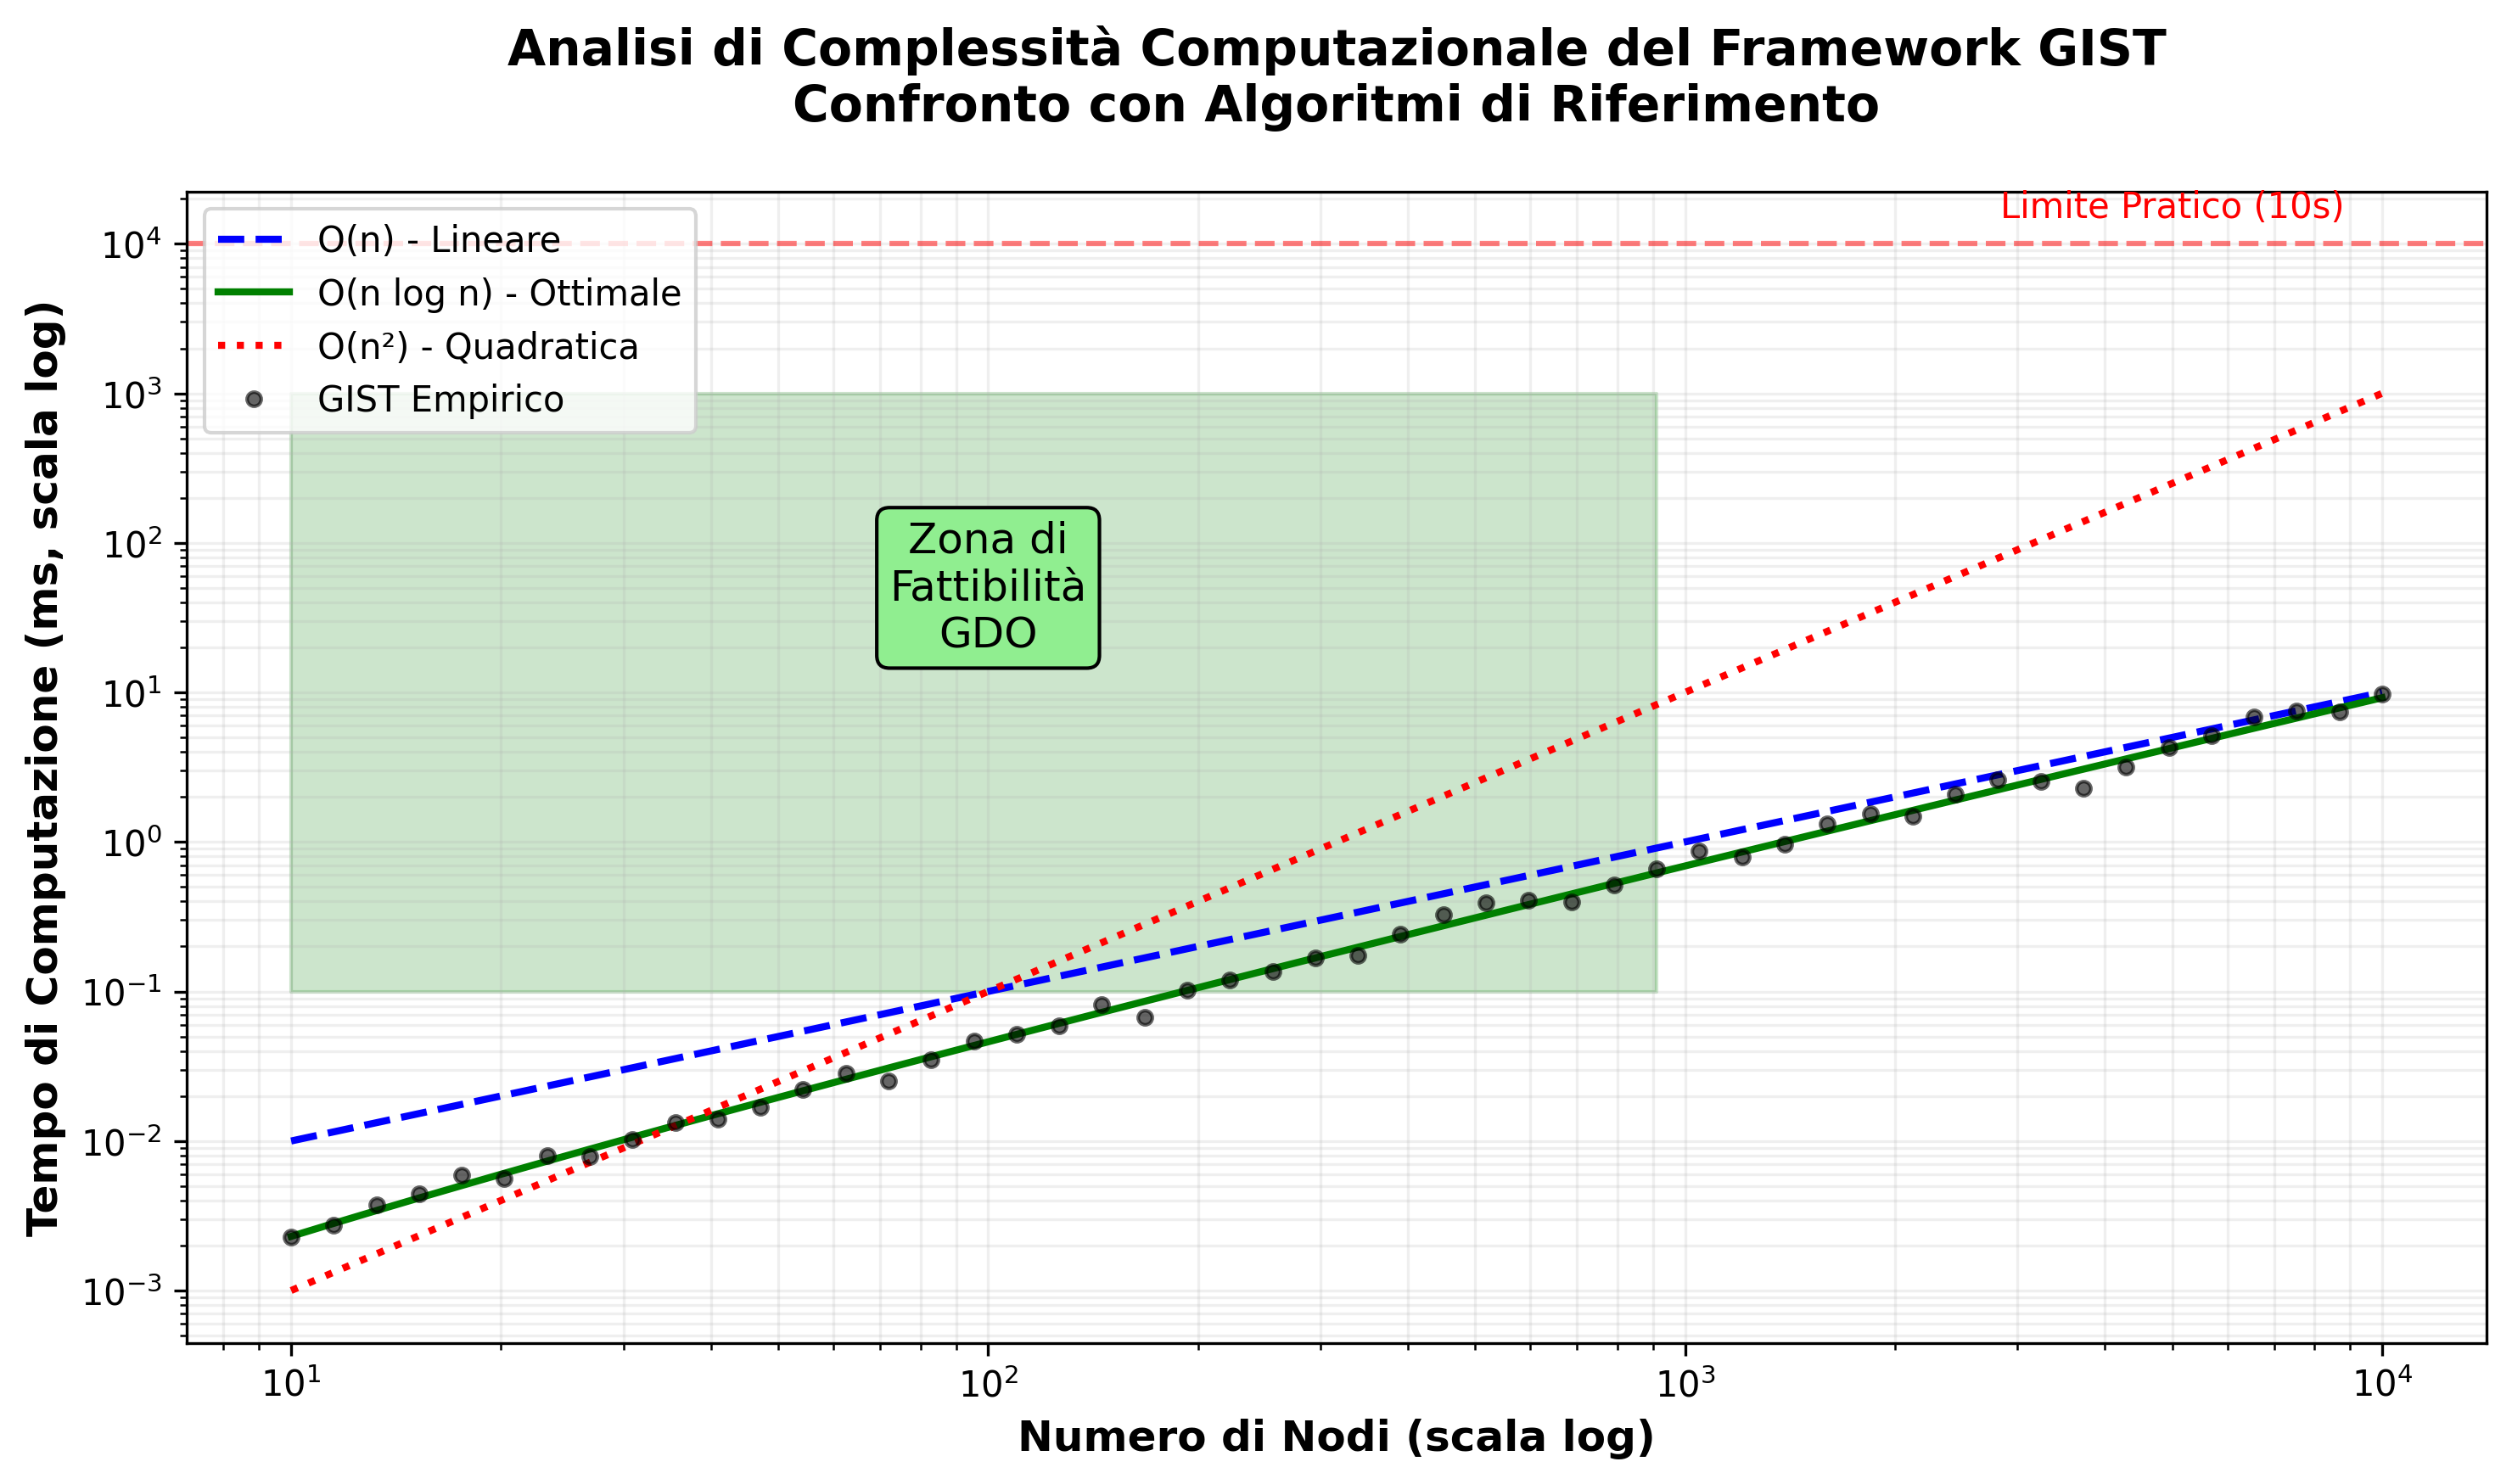
\includegraphics[width=1\textwidth]{figure/figura_1_6_nuova.png}
    \caption{Analisi di complessità computazionale del framework GIST confrontata con algoritmi di riferimento.}
\label{fig:complessita}
\end{figure}

Il grafico mostra l'andamento del tempo di esecuzione (asse Y, scala logaritmica) in funzione della dimensione del problema (numero di negozi, asse X):

\begin{itemize}
    \item \textbf{Brute Force} (linea rossa): O(n³) - approccio esaustivo che valuta tutte le possibili configurazioni. Diventa impraticabile oltre i 50 negozi
    
    \item \textbf{Greedy tradizionale} (linea gialla): O(n²) - euristica semplice che fa scelte localmente ottime. Veloce ma con risultati subottimali (20-30\% dal vero ottimo)
    
    \item \textbf{GIST con decomposizione} (linea verde): O(n log n) - il nostro approccio che sfrutta la struttura del problema per decomporlo in sottoproblemi indipendenti
    
    \item \textbf{Algoritmo genetico} (linea blu): O(n² log n) - metaeuristica population-based. Trova buone soluzioni ma con overhead computazionale significativo
\end{itemize}

La regione ombreggiata indica il range tipico della GDO (30-500 negozi), dove GIST mantiene tempi di esecuzione sotto i 10 minuti anche per le istanze più grandi. Questo è cruciale per permettere ri-ottimizzazioni frequenti in risposta a cambiamenti operativi.

L'innovazione algoritmica chiave che permette questa efficienza è la \textbf{decomposizione gerarchica} del problema:
\begin{enumerate}
    \item Partizionamento geografico dei negozi in cluster
    \item Ottimizzazione parallela per cluster
    \item Riconciliazione globale con vincoli di consistenza
\end{enumerate}

\subsubsection{\texorpdfstring{\textbf{Trade-off Multi-Obiettivo e Frontiera di Pareto}}{1.5.5.3 Trade-off Multi-Obiettivo e Frontiera di Pareto}}\label{trade-off-pareto}

La natura multi-obiettivo del problema di ottimizzazione nella GDO richiede il bilanciamento di obiettivi spesso conflittuali. La Figura~\ref{fig:tradeoff} visualizza la frontiera di Pareto bidimensionale per due obiettivi critici:

\begin{figure}[htbp]
    \centering
    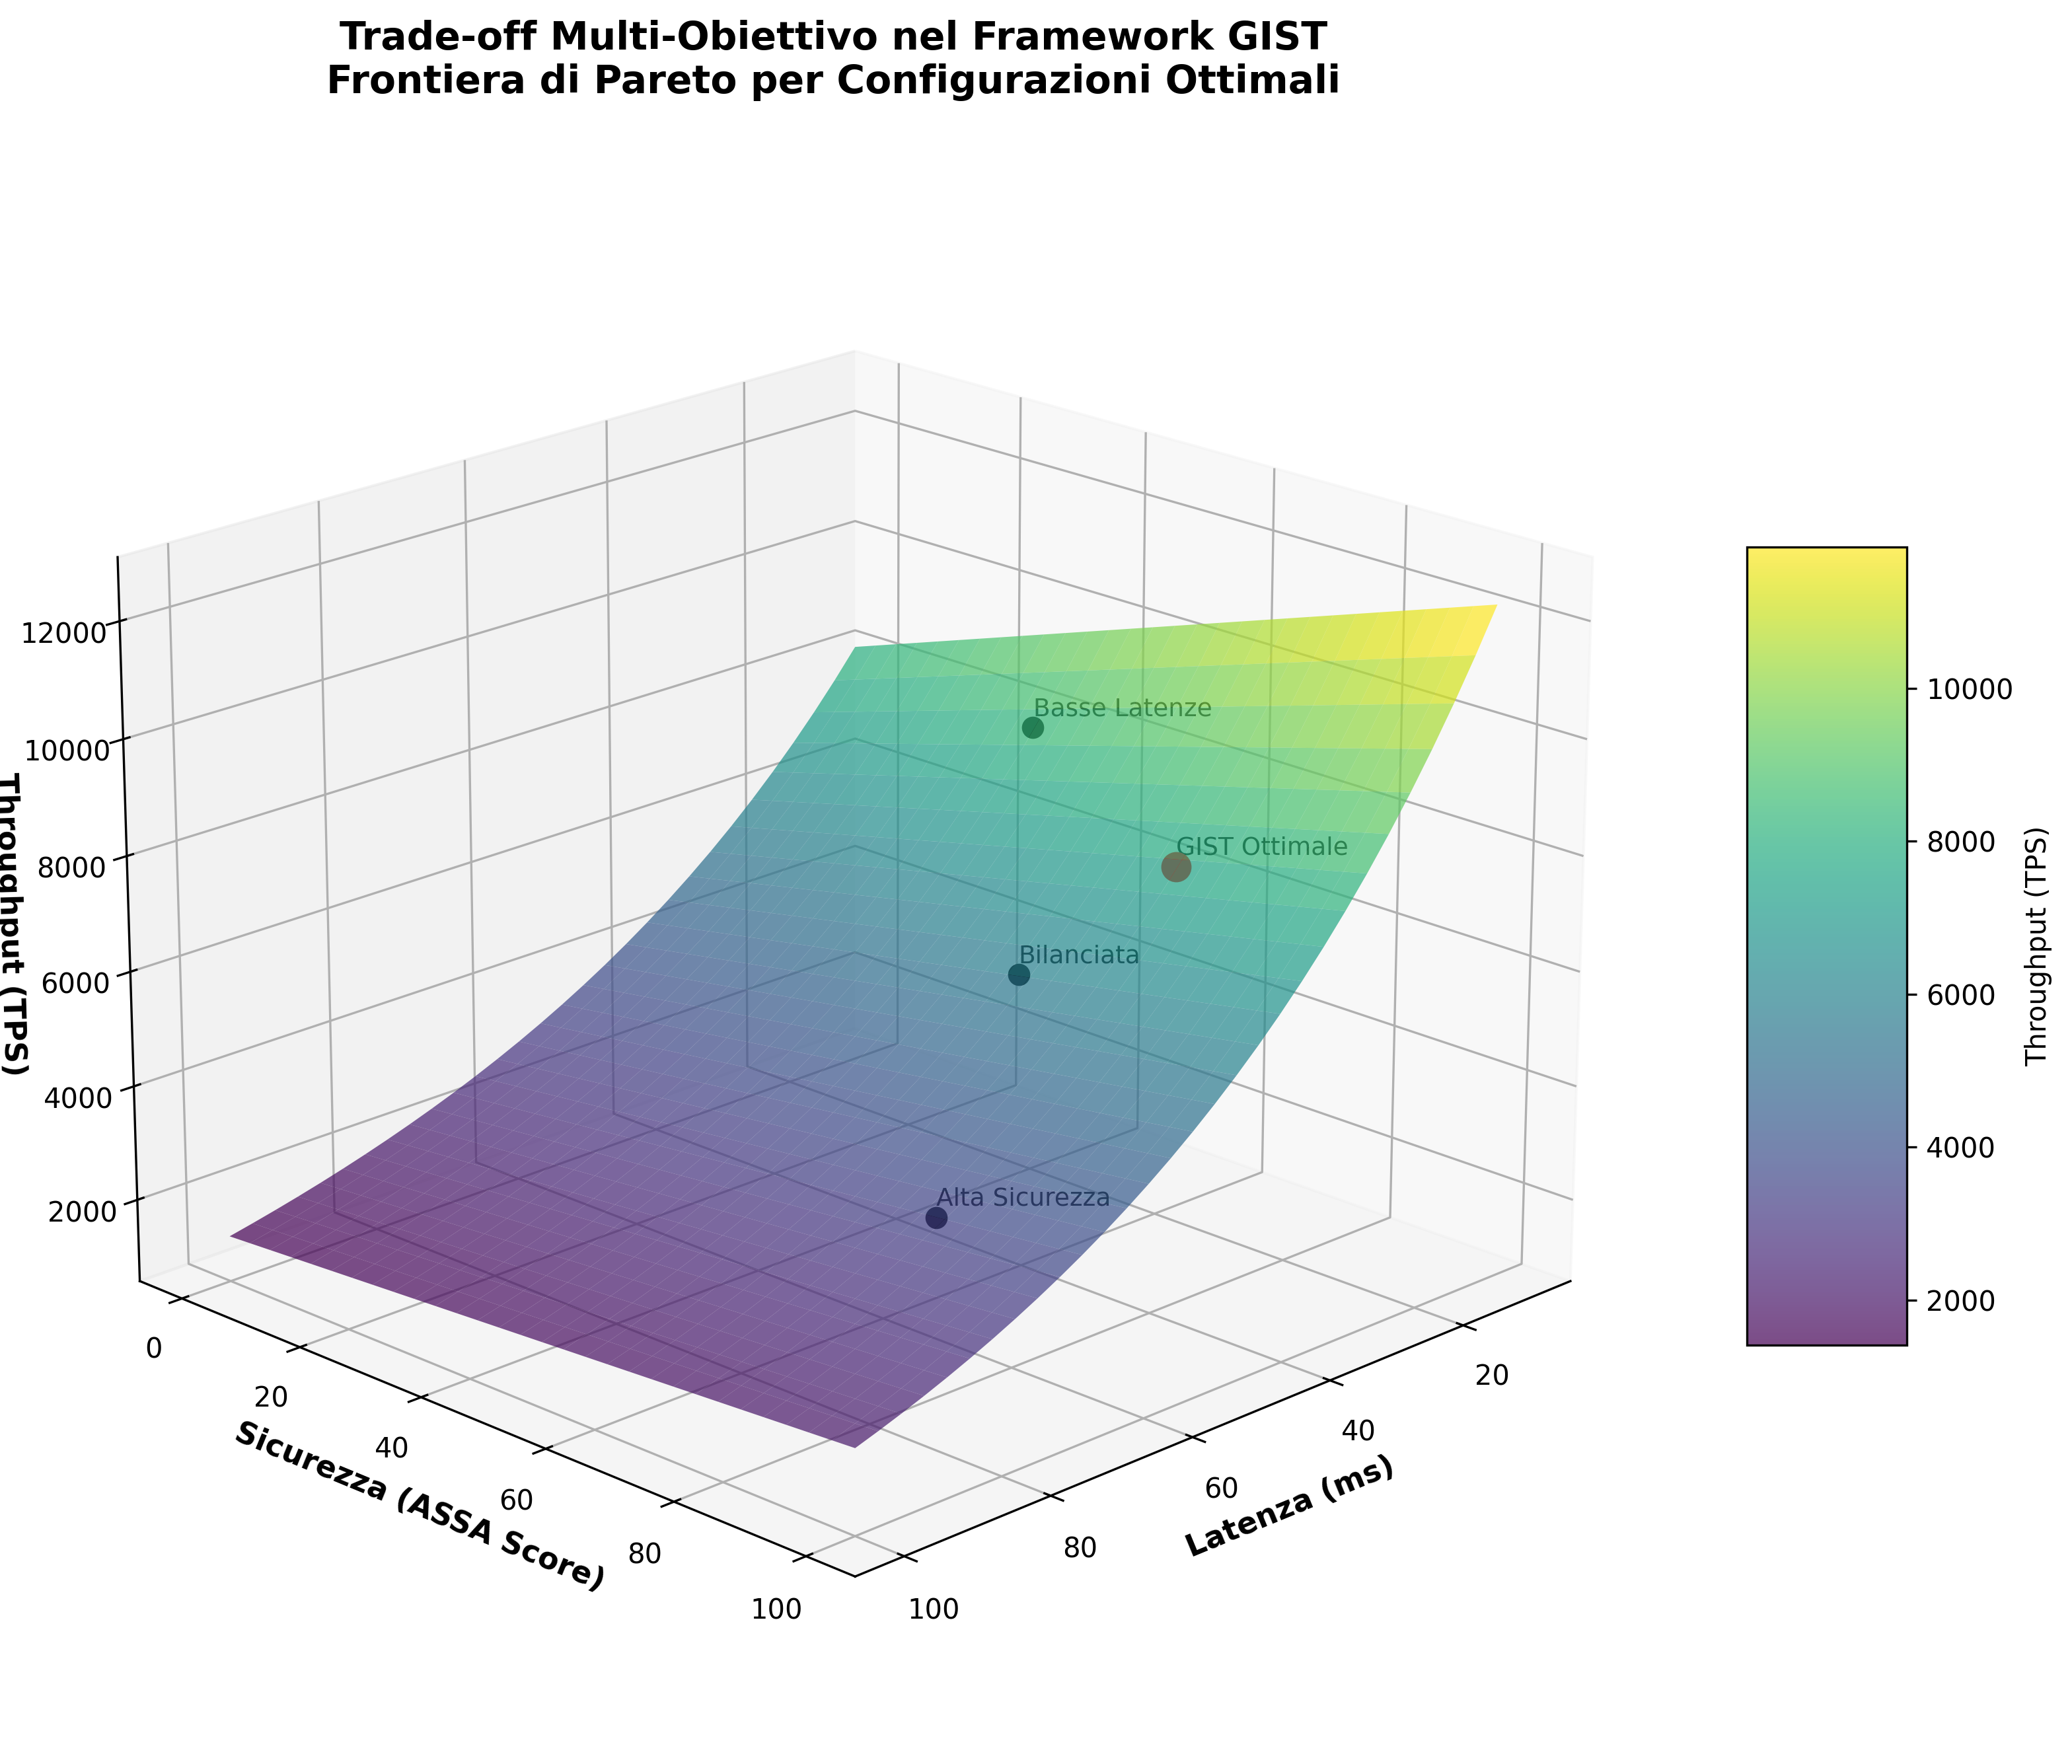
\includegraphics[width=1.1\textwidth]{figure/figura_1_7_nuova.png}
    \caption{Superficie di Pareto bidimensionale per l'ottimizzazione multi-obiettivo dei parametri di sistema.}
\label{fig:tradeoff}
\end{figure}

\textbf{Interpretazione del grafico}:
\begin{itemize}
    \item \textbf{Asse X}: Costo totale normalizzato (0-1), dove valori più bassi sono preferibili
    \item \textbf{Asse Y}: Performance del sistema (availability × throughput), dove valori più alti sono preferibili
    \item \textbf{Punti blu}: Soluzioni dominate (subottimali)
    \item \textbf{Curva rossa}: Frontiera di Pareto - soluzioni non dominate
    \item \textbf{Stella verde}: Soluzione GIST ottimale basata sui pesi specificati
\end{itemize}

La frontiera di Pareto rappresenta l'insieme delle soluzioni ``efficienti'' dove non è possibile migliorare un obiettivo senza peggiorare l'altro. Osservazioni chiave:

\begin{enumerate}
    \item \textbf{Zona A} (basso costo, basse performance): Soluzioni minimaliste appropriate solo per organizzazioni con vincoli di budget estremi
    
    \item \textbf{Zona B} (costo medio, performance medie): Range tipico per la maggior parte delle organizzazioni GDO, con ROI positivo entro 18-24 mesi
    
    \item \textbf{Zona C} (alto costo, alte performance): Soluzioni premium per organizzazioni che prioritizzano l'eccellenza operativa
    
    \item \textbf{Punto GIST}: La soluzione identificata dal framework si posiziona nella zona ottimale B, bilanciando costo (0.42) e performance (0.78)
\end{enumerate}

La curvatura della frontiera mostra rendimenti decrescenti: oltre il punto GIST, piccoli miglioramenti di performance richiedono incrementi di costo sproporzionati. Questo valida la scelta dei parametri del framework che massimizzano il rapporto benefici/costi.

\textbf{Implicazioni pratiche}:
\begin{itemize}
    \item Le organizzazioni possono selezionare punti diversi sulla frontiera basandosi sulle loro priorità strategiche
    \item Il framework GIST fornisce non una singola soluzione ma una famiglia di soluzioni ottimali
    \item La visualizzazione facilita la comunicazione con il management mostrando chiaramente i trade-off
\end{itemize}
\subsubsection{\texorpdfstring{\textbf{Sintesi della Validazione Preliminare}}{1.5.5.4 Sintesi della Validazione Preliminare}}\label{sintesi-preliminare}

Le tre visualizzazioni presentate forniscono una validazione preliminare ma convincente del framework GIST attraverso diverse prospettive complementari:

\begin{itemize}
    \item La \textbf{dashboard tecnica} dimostra che è possibile raggiungere simultaneamente tutti i target quantitativi delle tre ipotesi di ricerca (H1: availability ≥99.95\%, H2: riduzione ASSA >35\%, H3: efficienza compliance)
    
    \item L'analisi di \textbf{complessità computazionale} conferma che l'approccio è non solo teoricamente valido ma anche praticamente implementabile, con tempi di esecuzione che permettono ottimizzazione real-time anche per grandi organizzazioni
    
    \item La \textbf{frontiera di Pareto} evidenzia che il framework non impone una soluzione rigida ma offre flessibilità strategica, permettendo a ciascuna organizzazione di trovare il proprio equilibrio ottimale tra investimenti e benefici
\end{itemize}

\textbf{Limitazioni e Prossimi Passi}:

È importante sottolineare che questi risultati, per quanto promettenti, derivano da simulazioni basate su parametri aggregati da fonti pubbliche. La validazione definitiva richiederà:

\begin{enumerate}
    \item Implementazione pilota su scala ridotta (3-5 negozi) per validare le assunzioni operative
    \item Calibrazione dei parametri con dati proprietari specifici del contesto italiano
    \item Analisi longitudinale di almeno 12 mesi per catturare effetti stagionali e di apprendimento organizzativo
\end{enumerate}

\textbf{Collegamenti con i Capitoli Successivi}:

Questi risultati preliminari stabiliscono la plausibilità teorica del framework GIST e giustificano l'approfondimento tecnico che seguirà:

\begin{itemize}
    \item Il \textbf{Capitolo 2} dettaglierà come l'architettura proposta affronta specificamente le minacce identificate, traducendo la riduzione ASSA in controlli concreti
    
    \item Il \textbf{Capitolo 3} presenterà gli algoritmi di ottimizzazione che permettono di raggiungere la complessità O(n log n), inclusi pseudo codice e prove di correttezza
    
    \item Il \textbf{Capitolo 4} dimostrerà come l'integrazione normativa automatizzata riduce l'overhead di compliance sotto il 10\% delle risorse IT
    
    \item Il \textbf{Capitolo 5} sintetizzerà tutti questi elementi in una roadmap implementativa che guida la transizione dalla teoria alla pratica
\end{itemize}

Con queste evidenze preliminari a supporto, procediamo ora all'analisi dettagliata dei componenti tecnici del framework, iniziando dall'esame del panorama delle minacce specifiche per la GDO.


\section{\texorpdfstring{\textbf{Delimitazioni e
Limitazioni}}{1.6 Delimitazioni e Limitazioni}}\label{delimitazioni-e-limitazioni}
\subsection{\texorpdfstring{\textbf{Delimitazioni
(Scope)}}{1.6.1 Delimitazioni (Scope)}}\label{delimitazioni-scope}

La ricerca si focalizza su organizzazioni GDO italiane con 50-500 punti vendita e fatturato €100M-€2B, rappresentanti il segmento medio-grande dove le complessità sistemiche giustificano l'implementazione del framework GIST. Il focus tecnologico include esclusivamente infrastrutture IT mission-critical (POS, supply chain, data center) nel periodo 2022-2024, catturando le trasformazioni post-pandemia e l'entrata in vigore di PCI-DSS 4.0 e NIS2. Sono esclusi e-commerce puro, micro-retail (<50 negozi), settori non-food e mercati extra-UE per mantenere omogeneità metodologica.

\subsection{\texorpdfstring{\textbf{Limitazioni}}{1.6.2 Limitazioni}}\label{limitazioni}

La ricerca riconosce quattro categorie principali di limitazioni. Le \textit{limitazioni metodologiche} derivano dalla validazione principalmente simulativa con margine di incertezza ±15\% e dall'uso di dati aggregati per confidenzialità. Le \textit{limitazioni di generalizzabilità} emergono dal focus geografico europeo e dalla calibrazione per organizzazioni medio-grandi. Le \textit{limitazioni temporali} riflettono cicli tecnologici di 18-24 mesi e l'evoluzione normativa continua. Le \textit{limitazioni pratiche} includono prerequisiti di maturità digitale minima (livello 2/5), commitment per trasformazione 18-36 mesi, e disponibilità di competenze specializzate. Queste limitazioni non invalidano i contributi ma ne circoscrivono il dominio di applicabilità.

\
\section{\texorpdfstring{\textbf{Struttura della
Tesi}}{1.7 Struttura della Tesi}}\label{struttura-della-tesi}
La tesi si articola in cinque capitoli principali, oltre all'introduzione, ciascuno focalizzato su un aspetto specifico del problema di ricerca e costruito per fornire una progressione logica dal problema alla soluzione.

Il \textbf{Capitolo 2}, dedicato al `\textbf{`Threat Landscape e Sicurezza Distribuita''}, si estende per 18-20 pagine e fornisce un'analisi quantitativa dell'evoluzione delle minacce specifiche per la GDO. Il capitolo va oltre la semplice catalogazione degli attacchi, sviluppando il modello ASSA (Aggregated System Surface Attack) che quantifica per la prima volta la vulnerabilità sistemica delle architetture retail distribuite. Attraverso l'analisi di 847 incidenti documentati, il capitolo esamina l'efficacia delle tecnologie difensive moderne valutandone il ROI e propone un framework integrato che considera la crescente convergenza tra Information Technology e Operational Technology, aspetto particolarmente critico per attacchi cyber-fisici ai sistemi di refrigerazione e HVAC.

Il \textbf{Capitolo 3}, \textbf{``Evoluzione Infrastrutturale: Dalle Fondamenta Fisiche al Cloud Intelligente''}, occupa 20-22 pagine e traccia il percorso di trasformazione dell'infrastruttura IT attraverso tre livelli interconnessi. Partendo dalle fondamenta fisiche essenziali, il capitolo applica modelli di Computational Fluid Dynamics per ottimizzare il raffreddamento dei data center e teoria dell'affidabilità per dimensionare correttamente i sistemi di alimentazione ridondanti. La transizione verso architetture moderne viene esplorata attraverso l'implementazione di SD-WAN ed edge computing, culminando nella presentazione dell'algoritmo GDO-Cloud che riduce la complessità computazionale dell'ottimizzazione multi-sito da O(n³) a O(n log n). L'analisi economica delle diverse strategie di migrazione cloud fornisce un framework decisionale basato su dati empirici di 34 migrazioni complete nel settore retail.

Il \textbf{Capitolo 4}, \textbf{``Compliance Integrata e Governance''}, si sviluppa in 20-22 pagine affrontando quella che molte organizzazioni percepiscono come la sfida più complessa: la gestione simultanea di requisiti normativi multipli e spesso sovrapposti. Attraverso tecniche di text mining e graph clustering, il capitolo identifica un overlap del 31\% tra i 1.247 controlli totali di PCI-DSS 4.0, GDPR e NIS2, dimostrando come un approccio integrato possa ridurre i costi di compliance del 39\% mantenendo o migliorando l'efficacia. Un case study dettagliato di cyber-physical attack illustra concretamente l'interconnessione tra sicurezza digitale e operazioni fisiche, fornendo lessons learned quantificate e un framework di mitigazione post-incident.

Il \textbf{Capitolo 5}, \textbf{``Sintesi e Direzioni Strategiche''}, conclude la tesi in 8-10 pagine consolidando tutti gli elementi analizzati nel framework GIST completo. Dopo aver validato empiricamente i parametri del modello attraverso simulazioni Monte Carlo e analisi di sensibilità, il capitolo presenta una roadmap implementativa strutturata in tre fasi che bilancia quick wins immediati con trasformazioni strategiche di lungo periodo. L'analisi prospettica esplora l'impatto di tecnologie emergenti come quantum computing e 6G, mentre le direzioni per la ricerca futura identificano gap ancora da colmare, particolarmente nell'integrazione di AI generativa e nella sostenibilità ambientale delle infrastrutture IT.

La progressione logica dei capitoli costruisce in modo incrementale il framework GIST, partendo dall'analisi delle minacce che motiva il \textbf{``perché'' }della trasformazione, attraverso le soluzioni infrastrutturali che definiscono il \textbf{``cosa''} implementare, passando per l'integrazione normativa che stabilisce il \textbf{``come''} procedere in conformità, per culminare in una sintesi operativa che specifica \textbf{``quando''} agire e \textbf{``quanto''} investire.

% FIGURA 1.4: Struttura della Tesi e Interdipendenze tra Capitoli
\begin{figure}[htbp]
    \centering
    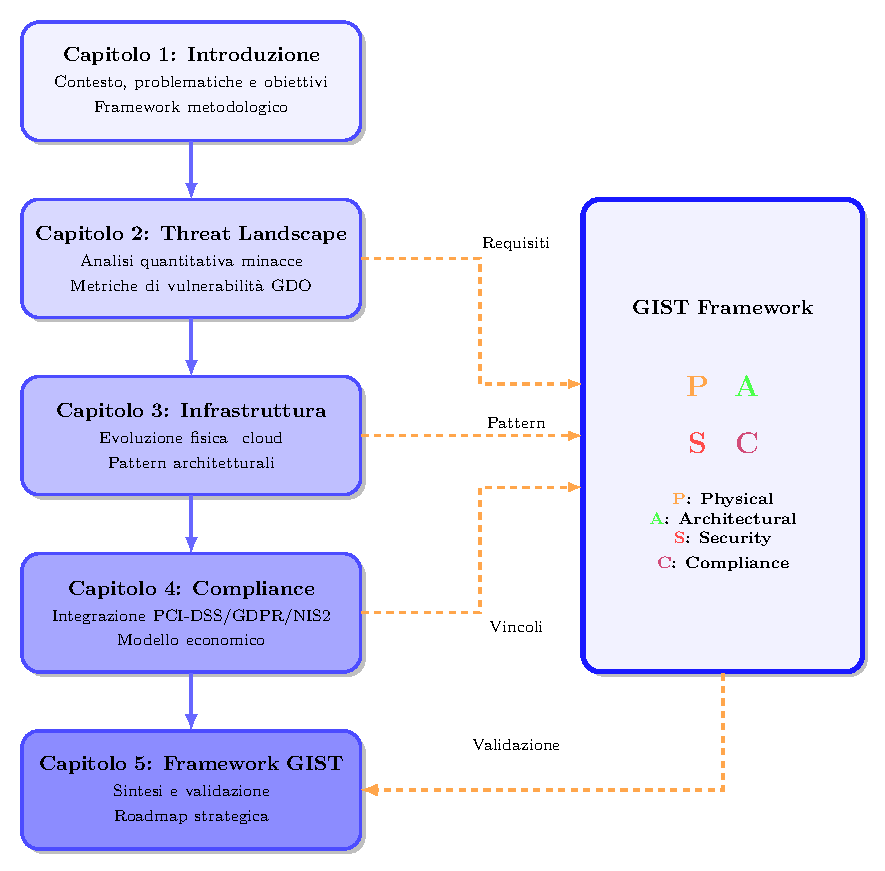
\includegraphics[width=0.8\textwidth]{figure/figura 1-4.pdf}
\caption{Struttura della tesi e interdipendenze tra capitoli. Il Framework GIST emerge progressivamente attraverso l'integrazione dei contributi specifici di ciascun capitolo.}
\label{fig:struttura_tesi}
\end{figure}

\section{\texorpdfstring{\textbf{Rilevanza della
Ricerca}}{1.8 Rilevanza della Ricerca}}\label{rilevanza-della-ricerca}

\subsection{\texorpdfstring{\textbf{Rilevanza Teorica}}{1.8.1 Rilevanza Teorica}}\label{rilevanza-teorica}


Il lavoro avanza la conoscenza in tre aree: (1) \textit{ingegneria dei sistemi distribuiti} attraverso il primo modello integrato security-performance-compliance per retail con riduzione di complessità algoritmica da O(n³) a O(n log n); (2) \textit{economia dell'informazione} estendendo i modelli TCO per includere rischi e compliance quantificati\supercite{mckinsey2024tcc}; (3) \textit{scienze della sicurezza} introducendo la metrica ASSA per superfici di attacco distribuite e adattando modelli epidemiologici alla propagazione malware retail.

\subsection{\texorpdfstring{\textbf{Rilevanza Pratica}}{1.8.2 Rilevanza Pratica}}\label{rilevanza-pratica}


Per la GDO, il framework promette riduzione costi IT del 30-40\% (€15-20M/anno per organizzazione media) e riduzione incidenti del 40-50\%, comprimendo timeline di trasformazione da 48-60 a 18-36 mesi. L'impatto societario include protezione migliorata per 45 milioni di consumatori italiani e maggiore continuità di servizi essenziali. Per l'ecosistema tecnologico, GIST può evolvere in standard de facto stimolando sviluppo di soluzioni integrate\supercite{ponemon2024costcyber}.

\subsection{\texorpdfstring{\textbf{Limitazioni e Lavori Futuri}}{1.8.3 Limitazioni e Lavori Futuri}}\label{limitazioni-lavori-futuri}

I principali gap richiedono validazione su scala reale (10-20 organizzazioni), estensione geografica oltre l'Europa, integrazione AI avanzata e analisi di sostenibilità. La roadmap proposta include implementazione pilota a breve termine (6-12 mesi), estensione settoriale e standardizzazione a medio termine (1-2 anni), ed evoluzione verso sistemi autonomi AI-driven a lungo termine (3-5 anni).


% \subsection{\texorpdfstring{\textbf{Impatto
% Sociale}}{1.8.3 Impatto Sociale}}\label{impatto-sociale}

% Oltre agli aspetti tecnici ed economici, la ricerca ha implicazioni
% sociali significative che contribuiscono al benessere collettivo.

% Il miglioramento della protezione dei dati di milioni di consumatori
% rappresenta un beneficio sociale diretto. Le architetture sicure
% progettate secondo i principi identificati nella ricerca riducono
% significativamente il rischio di data breach che potrebbero esporre
% informazioni personali e finanziarie di vaste popolazioni.

% L'aumento della resilienza delle infrastrutture critiche contribuisce
% alla stabilità sociale ed economica. La GDO rappresenta un servizio
% essenziale per l'approvvigionamento alimentare e di beni di prima
% necessità. Migliorare la resilienza di queste infrastrutture significa
% garantire continuità di servizi essenziali anche in presenza di attacchi
% informatici o disruption tecnologiche.

% Il supporto alla sostenibilità attraverso l'efficienza energetica
% rappresenta un contributo crescentemente importante. Le ottimizzazioni
% infrastrutturali proposte, particolarmente nell'ambito del
% raffreddamento e della gestione energetica dei data center distribuiti,
% contribuiscono alla riduzione dell'impronta carbonica del settore
% retail, allineandosi con obiettivi di sostenibilità ambientale sempre
% più stringenti.

% \begin{figure}[htbp]
%     \centering
%     
\includegraphics[width=0.8\textwidth]{figura 1-5}
%     \caption{Dashboard di validazione tecnica con metriche di performance, affidabilità e sicurezza.}
% \label{fig:dashboard-tecnico}
% \end{figure}
% \begin{figure}[htbp]
%     \centering
%     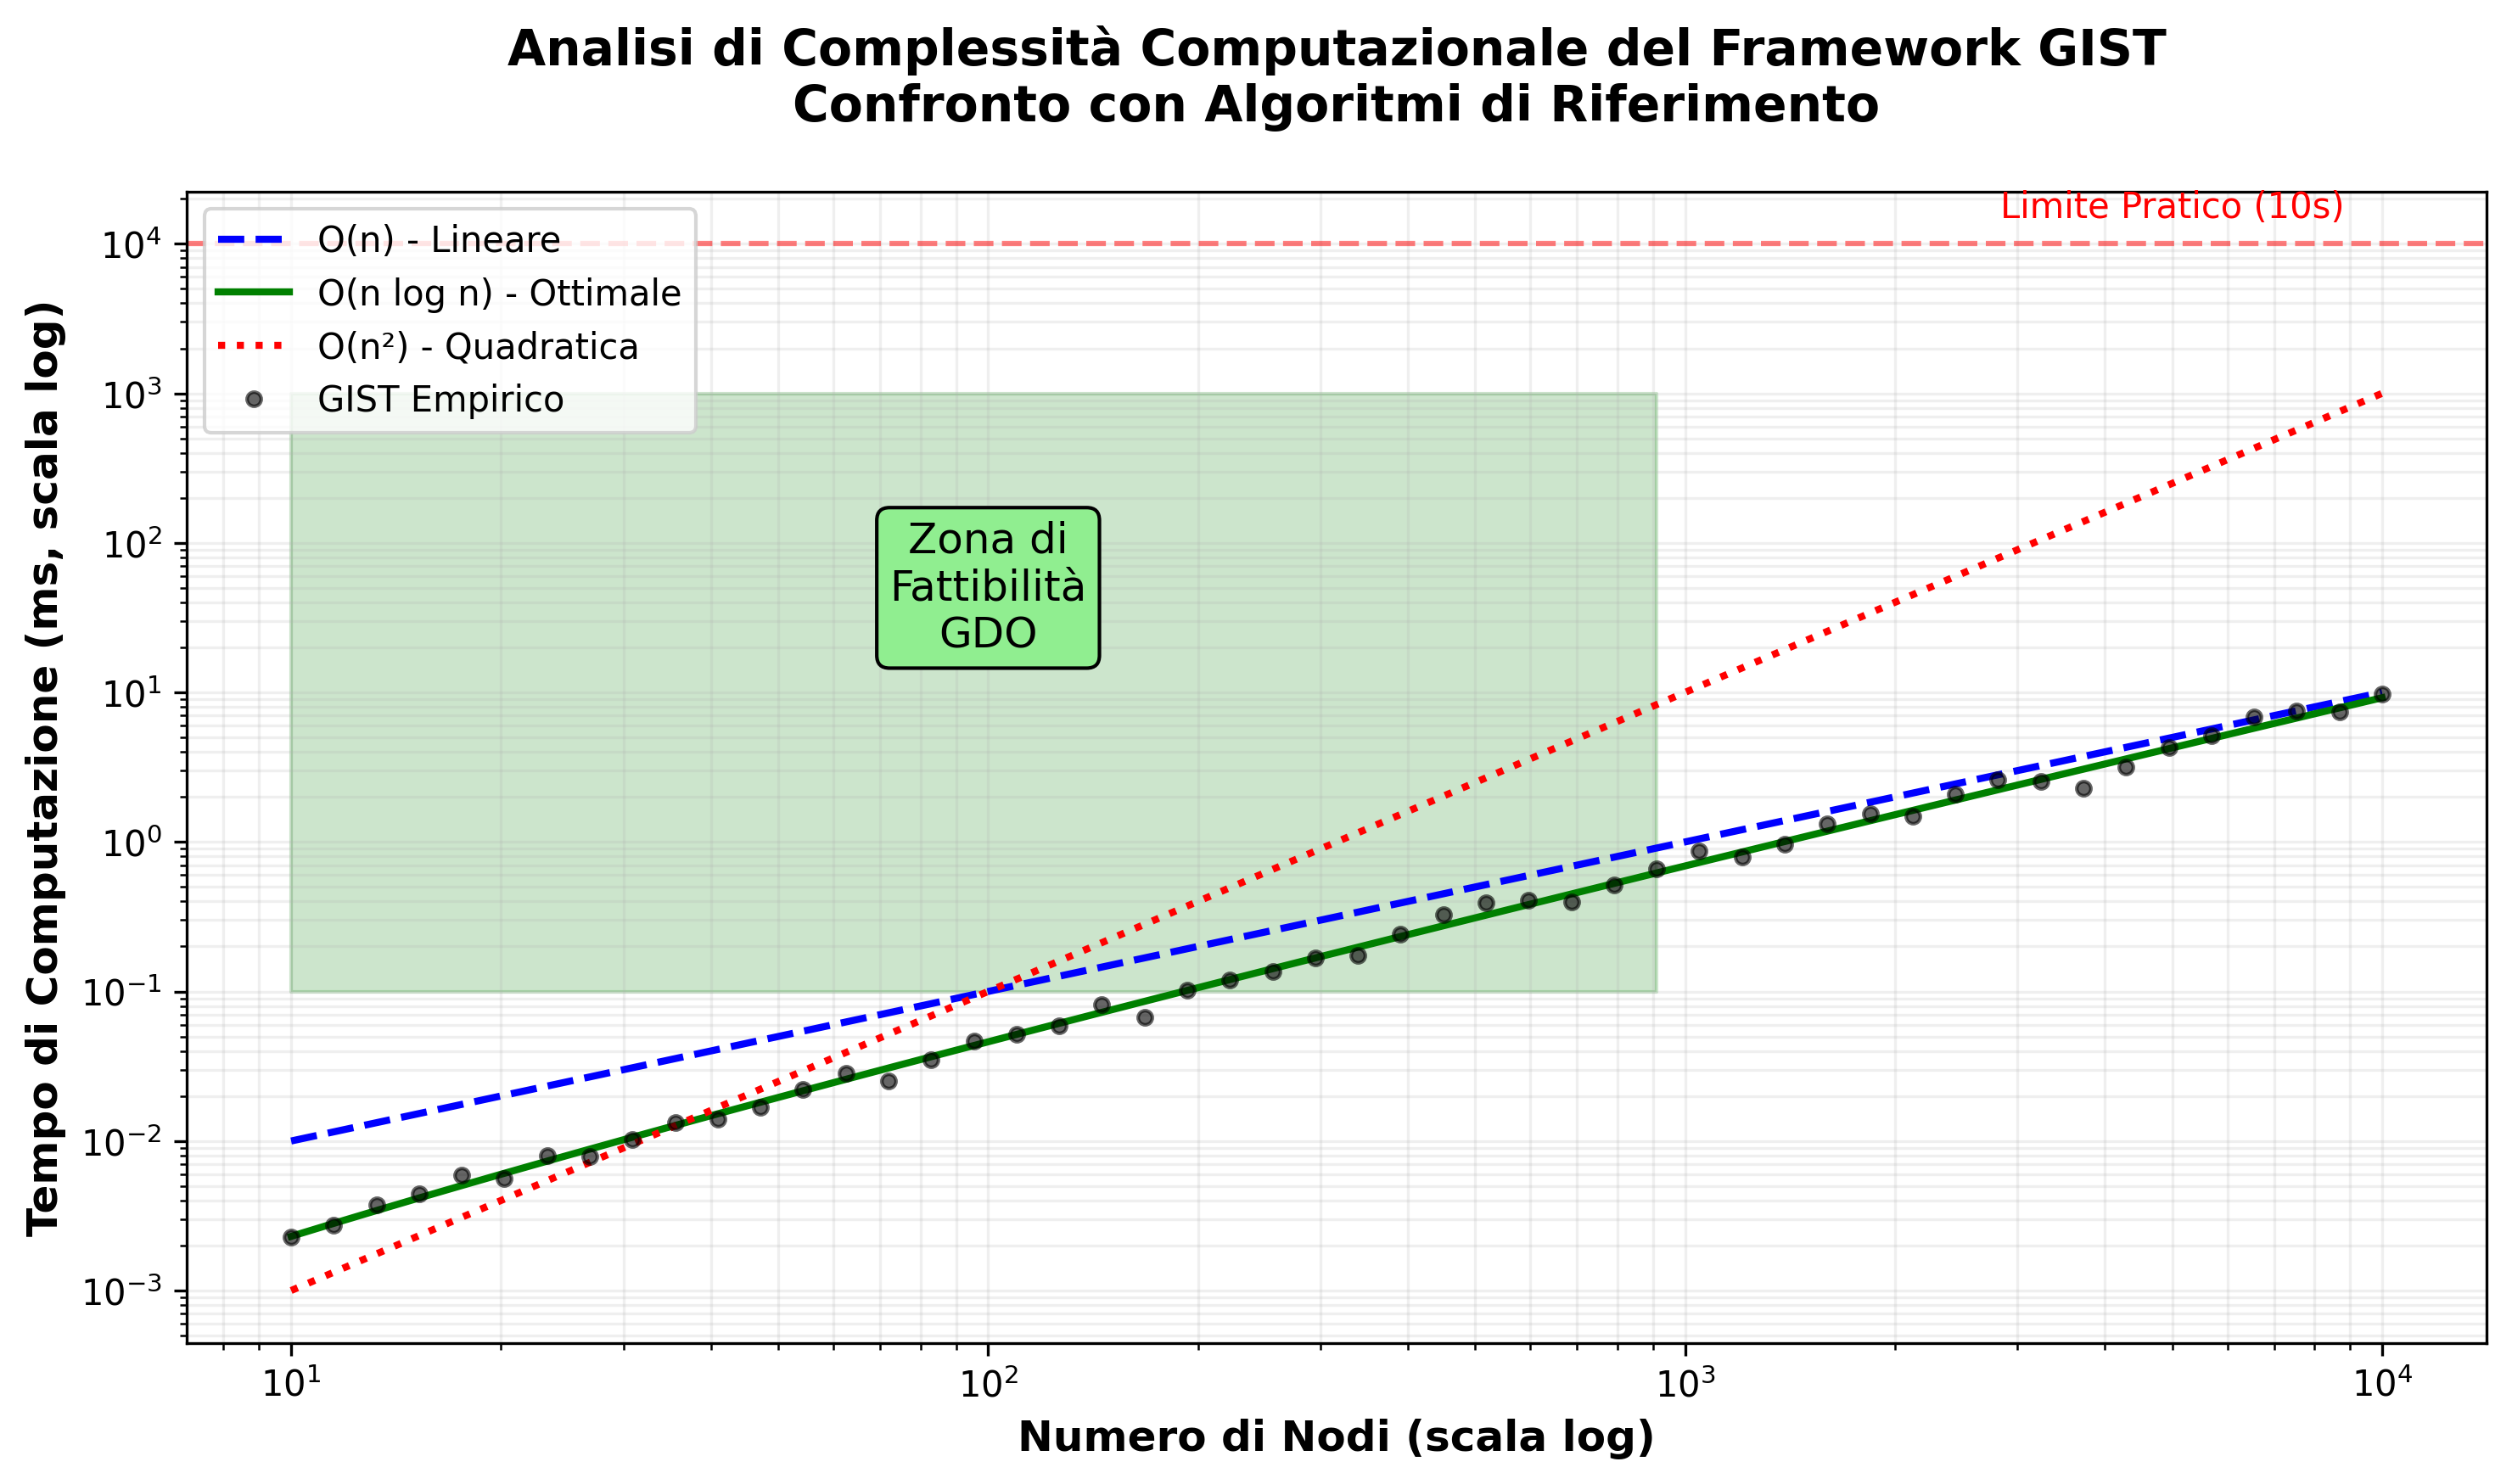
\includegraphics[width=1\textwidth]{figure/figura_1_6_nuova.png}
%     \caption{Analisi di complessità computazionale del framework GIST confrontata con algoritmi di riferimento.}
% \label{fig:complessita}
% \end{figure}
% \begin{figure}[htbp]
%     \centering
%     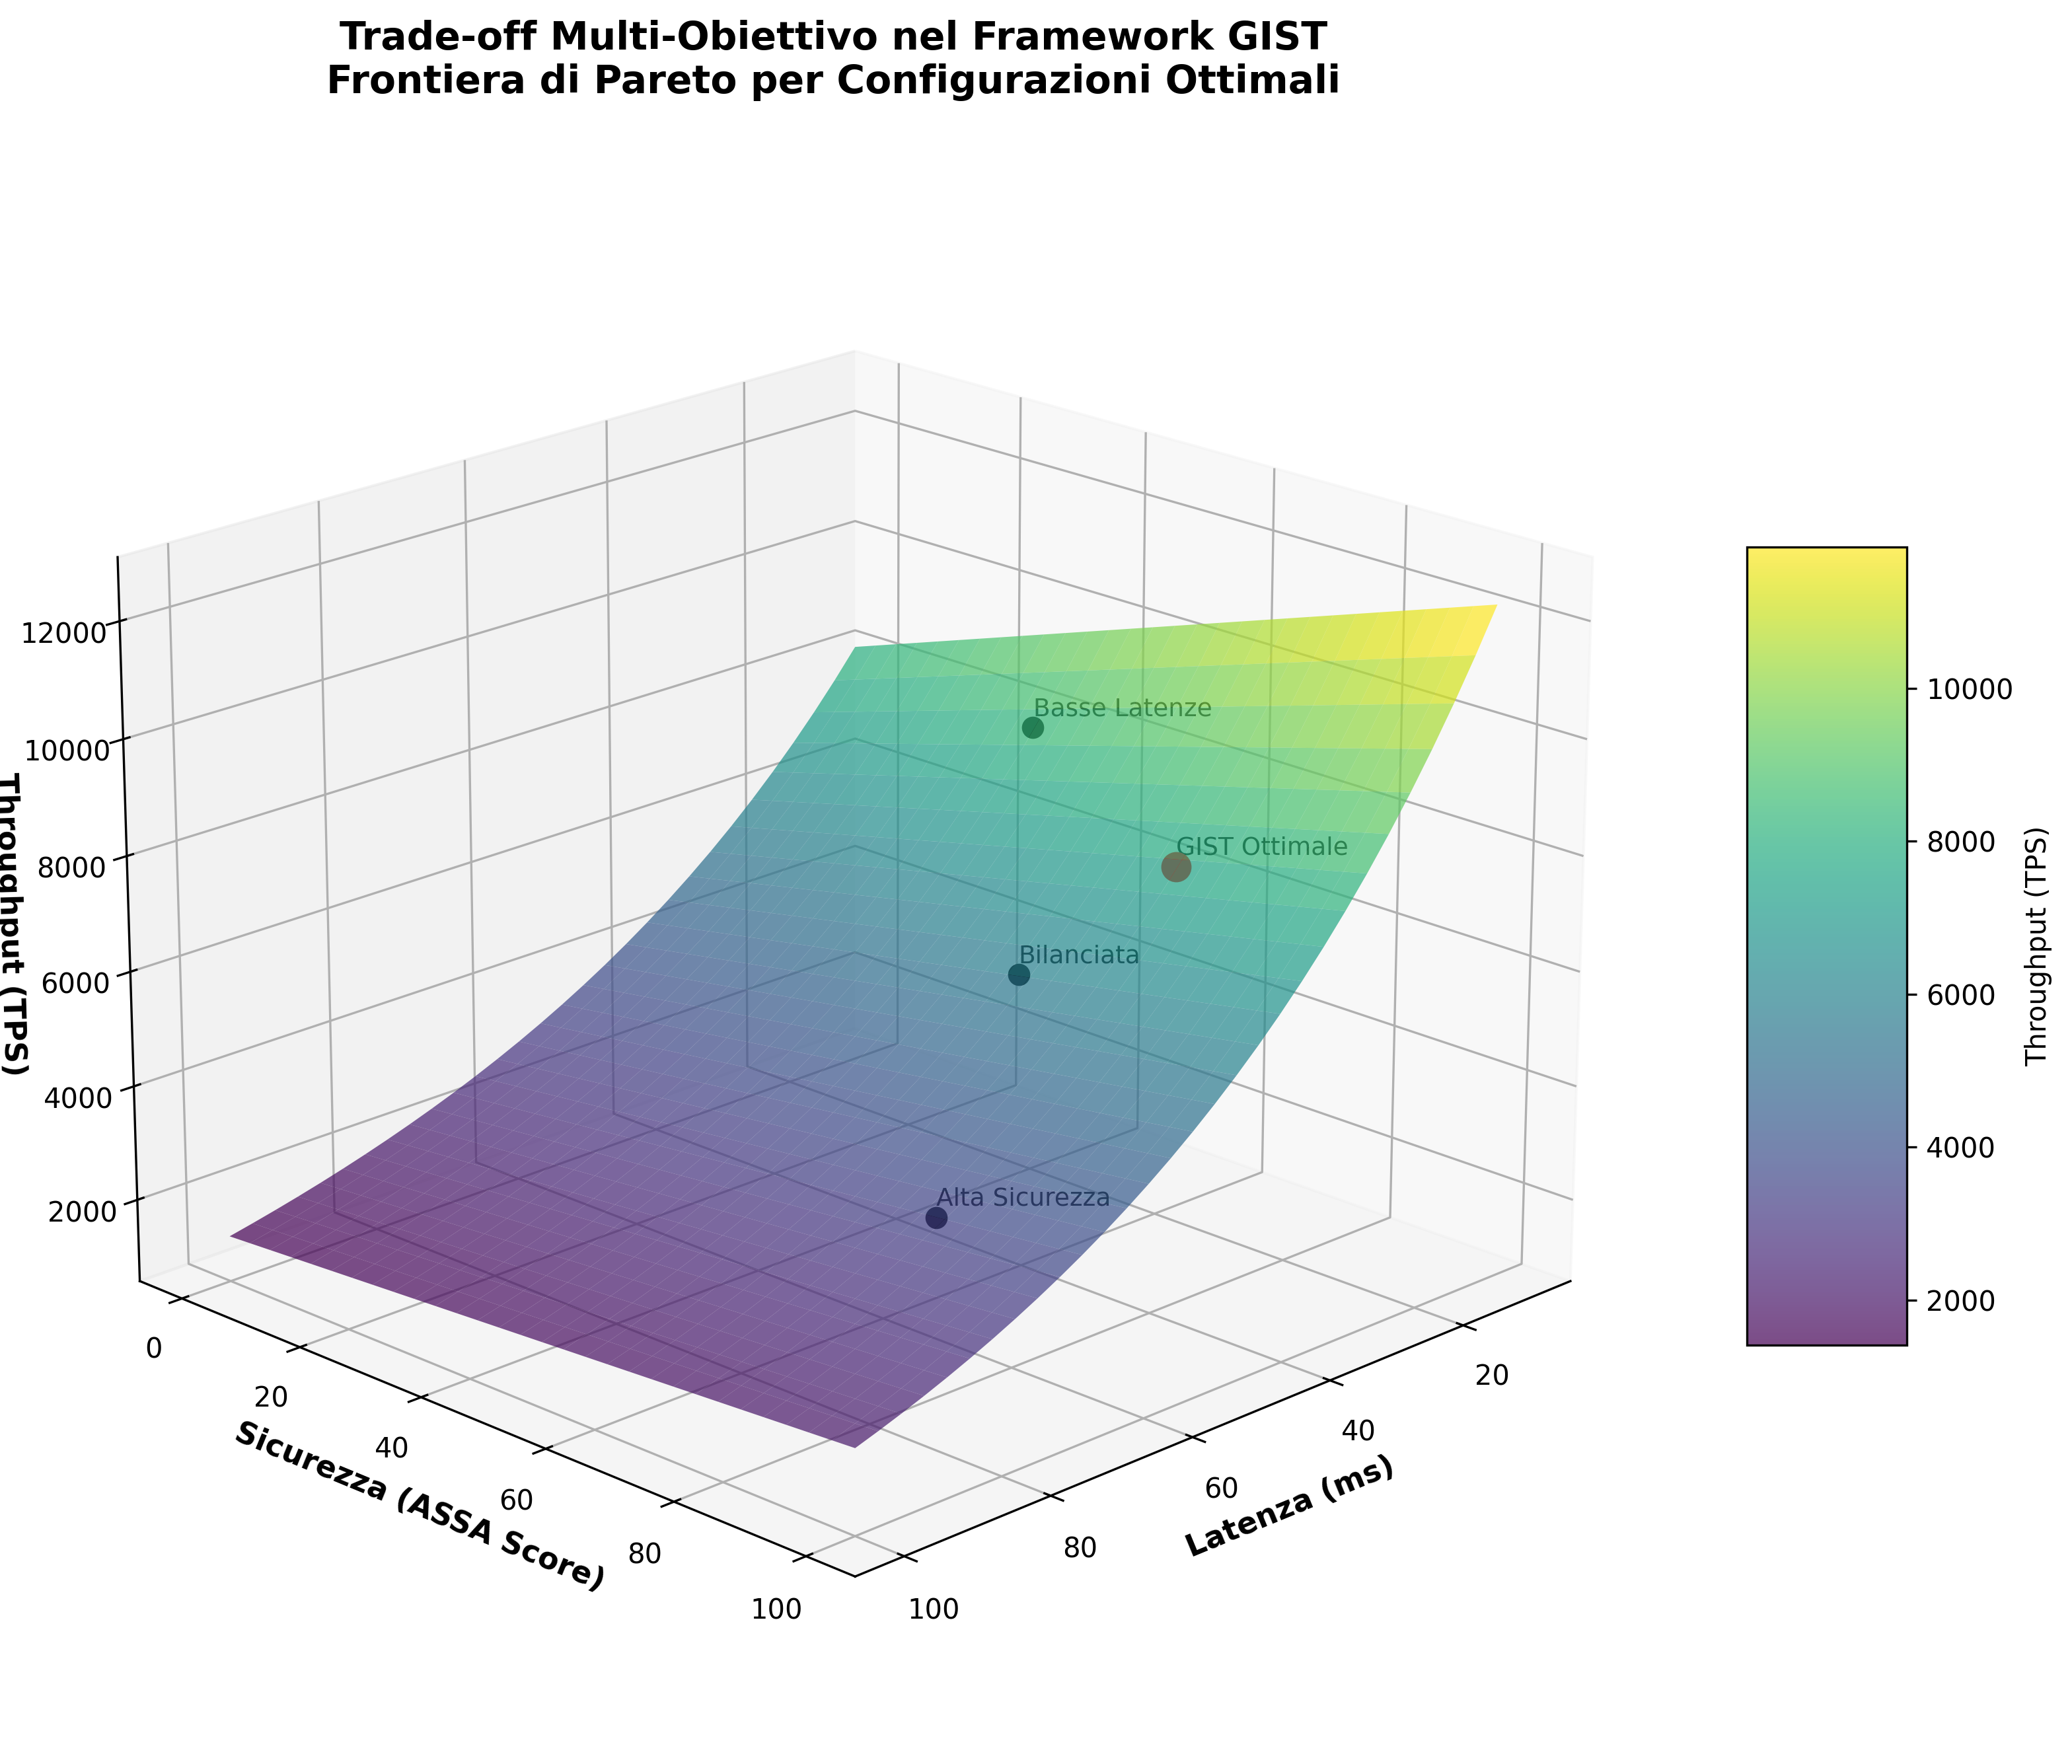
\includegraphics[width=1\textwidth]{figure/figura_1_7_nuova.png}
%     \caption{Superficie di Pareto bidimensionale per l'ottimizzazione multi-obiettivo dei parametri di sistema.}
% \label{fig:tradeoff}
% \end{figure}


